% This is the aspauthor.tex LaTeX file
% Copyright 2010, Astronomical Society of the Pacific Conference Series

\documentclass[11pt,twoside]{article}
\usepackage{asp2010}

\resetcounters

%\bibliographystyle{asp2010}

\markboth{Araya, Solar, Mardones, and Hochf\"arber}{Synthetic Data Cubes for Big
Data Algorithms}

\begin{document}

\title{Exorcising the Ghost in the Machine: Synthetic Spectral Data Cubes for
Assessing Big Data Algorithms}
\author{Mauricio~Araya$^1$, Mauricio~Solar$^1$, Diego Mardones$^2$ and Teodoro
Hochf�rber$^1$}
\affil{$^1$Universidad T\'ecnica Federico Santa Mar\'ia, Avenida Espa\~na 1680,
Casilla 110-V, Valpara\'iso, Chile.}
\affil{$^2$Universidad de Chile, Camino El Observatorio 1515, Las Condes, Santiago}

\begin{abstract}
The size and quantity of the data that is being generated by large astronomical
projects like ALMA, requires a paradigm change in astronomical data analysis.
Complex data, such as highly sensitive spectroscopic data in the form of large
data cubes, are not only difficult to manage, transfer and visualize, but they
also turn unfeasible the use of traditional data analysis techniques and
algorithms. Consequently, the attention have been placed on machine learning and
artificial intelligence techniques, to develop approximate and adaptive methods
for astronomical data analysis within a reasonable computational time.
Unfortunately, these techniques are usually sub optimal, stochastic and strongly
dependent of the parameters, which could easily turn into "a ghost in the
machine" for astronomers and practitioners. Therefore, a proper assessment of
these methods is not only desirable but mandatory for trusting them in
large-scale usage. The problem is that positively verifiable results are scarce
in astronomy, and moreover, science using bleeding-edge instrumentation
naturally lacks of reference values. We propose an Astronomical SYnthetic Data
Observations (ASYDO), a virtual service that generates synthetic spectroscopic
data in the form of data cubes. The objective of the tool is not to produce
accurate astrophysical simulations, but to generate a large number of labelled
synthetic data, to assess advanced computing algorithms for astronomy and to
develop novel Big Data algorithms. The synthetic data is generated using a set
of spectral lines, template functions for spatial and spectral distributions,
and simple models that produce reasonable synthetic observations. Emission lines
are obtained automatically using IVOA's SLAP protocol (or from a relational
database) and their spectral profiles correspond to distributions in the
exponential family. The spatial distributions correspond to simple functions
(e.g., 2D Gaussian), or to scalable template objects. The intensity, broadening
and radial velocity of each line is given by very simple and naive physical
models, yet ASYDO's generic implementation supports new user-made models, which
potentially allows adding more realistic simulations. The resulting data cube is
saved as a FITS file, also including all the tables and images used for
generating the cube. We expect to implement ASYDO as a virtual observatory
service in the near future.
\end{abstract}

\section{The Big Data Challenge}

The data deluge problem in astronomy is rapidly moving from a forecast to a
reality. Analyzing Astronomical Big Data (ABD) imposes new technological and
scientific challenges for astronomers that are not yet fully understood, meanwhile
massive astronomical datasets are starting to pile. There
is a growing consensus in the community that machine/statistical
learning and artificial intelligence techniques could be the key to cope with ABD, 
as they have been successfully applied in other Big Data domains such as biology and
finance. A common misconception when using these techniques is to think of them
as black-box machines, leading most of the times to mediocre results.
Therefore, a good integration of these techniques to astronomical data analysis
needs not only a proper understanding of the theory behind these methods, but
also a mechanism to assess the quality of the results, in order to perform a
correct parameter selection and to tailor ad-hoc methods to the problem at hand.

%In particular, learning algorithms are highly data consuming in their raw state, 
%but this can be significantly lightened as we encode prior knowledge in our model. 
%On the other hand, including too strong priors can lead to a very poor learning rate.
%A similar dilemma is the algorithm's flexibility, where more general methods
%require to setup more free parameters. These and other similar issues can be
%overwhelming for an astronomer, in the sense that most of these parameters 
%are not in the astrophysical domain, but in the abstract space of the method
%parameters. Moreover, verifiable and labelled real 
%data is scarce in astronomy, which is a problem for applying supervised methods
%and for performing parameter sensitivity analysis. Another common problem is
%the curse of dimensionality, which means that techniques that works well
%in few dimensions or samples, do not generally scale up directly. Consequently,
%the use of heuristic and approximate methods, usually with a strong stochastic
%component, is a common practice in machine learning and artificial intelligence.
%All these problems, can easily generate the sense of a ``ghost in the machine'' 
%for practitioners, which can lead to discarding useful methods due to the lack
%of a proper test bench.

To tackle this issue, we propose generating synthetic astronomical data,
not for performing accurate astrophysical simulations, but to test and evaluate 
complex algorithms and their parameters. The key idea is to use mock
astrophysical models to generate a huge amount of data (ABD) that resembles 
real observations in terms of dimensionality, sparseness and complexity.

\section{Synthetic Spectroscopic Data Cubes}

The Atacama Large Millimeter/Submillimeter Array (ALMA) is currently generating
observations that clearly qualify as ABD, at least in the terms of
dimensionality and complexity. The main data products after correlation and
calibration are high resolution spectroscopic data cubes, which are not only
difficult to manage and visualize, but they also carry complex information about
the molecules of one or several sources, and their dynamics in the form of emission lines.

A simple way to generate a synthetic cube is to use the following model for
a temperature of data cell:
\begin{equation}
C(x,y,f)=\sum_{l \in \mathcal{L}(x,y,f)}
\int_{\nu_f - \Delta
\nu/2}^{\nu_f + \Delta \nu/2} 
Br(\nu,l)df + \epsilon,
\label{eq:base}
\end{equation}
where $x$ and $y$ are spatial indices and $f$ is a spectral index 
in the cube. For each line $l$ that emits in the field of view of that cell, 
there is a specific broadening function that sums accordingly to the spectral
resolution $\Delta \nu$ for that frequency. An $epsilon$ Gaussian noise is added also
to the model.

For example, by assuming a simple Gaussian profile for all the lines, the model
would be:
\begin{equation}
C(x,y,f)=\sum_{l \in \mathcal{L}(x,y,f,l)}
\int_{\nu_f - \Delta
\nu/2}^{\nu_f + \Delta \nu/2} 
\frac{T_l(x,y)}{S_l(x,y) \sqrt{2\pi}}exp\left(- \frac{(\nu - \nu_l(1 +
Z_l(x,y)))^2}{2S_l(x,y)^2}\right) df +
\epsilon
\label{eq:base}
\end{equation}
where $T_l$ is the intensity matrix, $S_l$ the broadening matrix
(variance), and $Z_l$ the red-shift matrix of the line $l$. 
In practice, lines can be grouped by molecules and their
relative intensity can be randomly generated within reasonable
ranges obtained from the line's energy levels. Due to space constraints
the details of the models used for generating these emission lines
are not presented in this paper, but their are simplified versions of 
\cite{}

\subsection{The ASYDO Package}

The Astronomical SYnthetic Data Observations tool (ASYDO), is
a python package that generates arbitrary spectroscopic data cubes
in the ALMA bands, based on mock astrophysical models.
%The package is strongly based on scientific packages such as
%numpy, scipy and astropy. 

ASYDO works under the Virtual Universe (VU) concept, which is
a persistent object that can hold several sources spread in a virtual
celestial sphere. Sources that belongs to this universe 
are defined by a central coordinate ($\alpha_S$, $\delta_S$) and a base
red-shift $z_S$.
Each source can contain one or more components,
and each component uses one of the predefined astrophysical mock models (see
Figure~\ref{}). 

\begin{figure}
\begin{minipage}{0.3\linewidth}
\centerline{a)}
\centerline{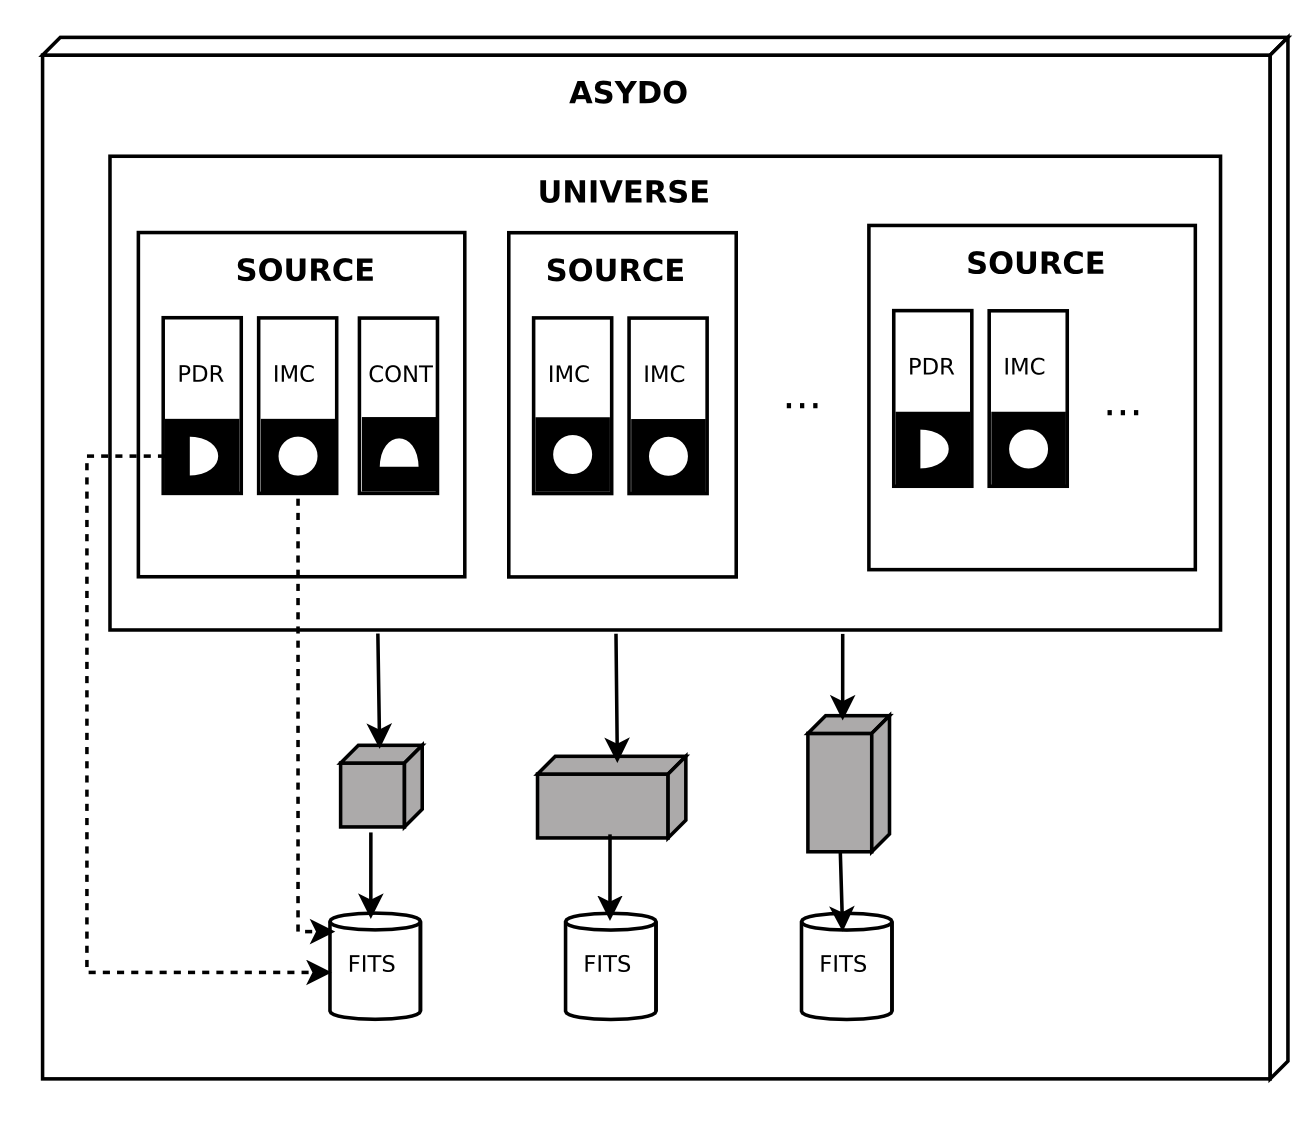
\includegraphics[width=0.9\linewidth]{internal.png}}
\end{minipage}
\begin{minipage}{0.3\linewidth}
\centerline{b)}
\centerline{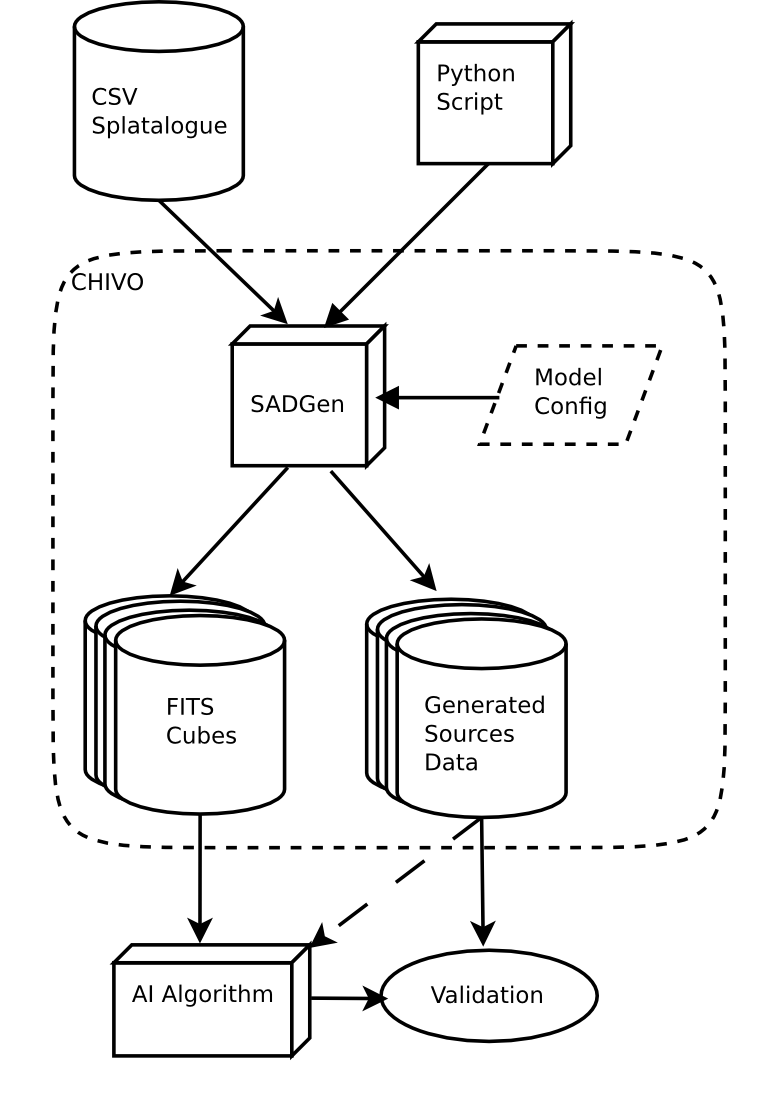
\includegraphics[width=0.7\linewidth]{archi.png}}
\end{minipage}
\begin{minipage}{0.3\linewidth}
\centerline{b)}
\centerline{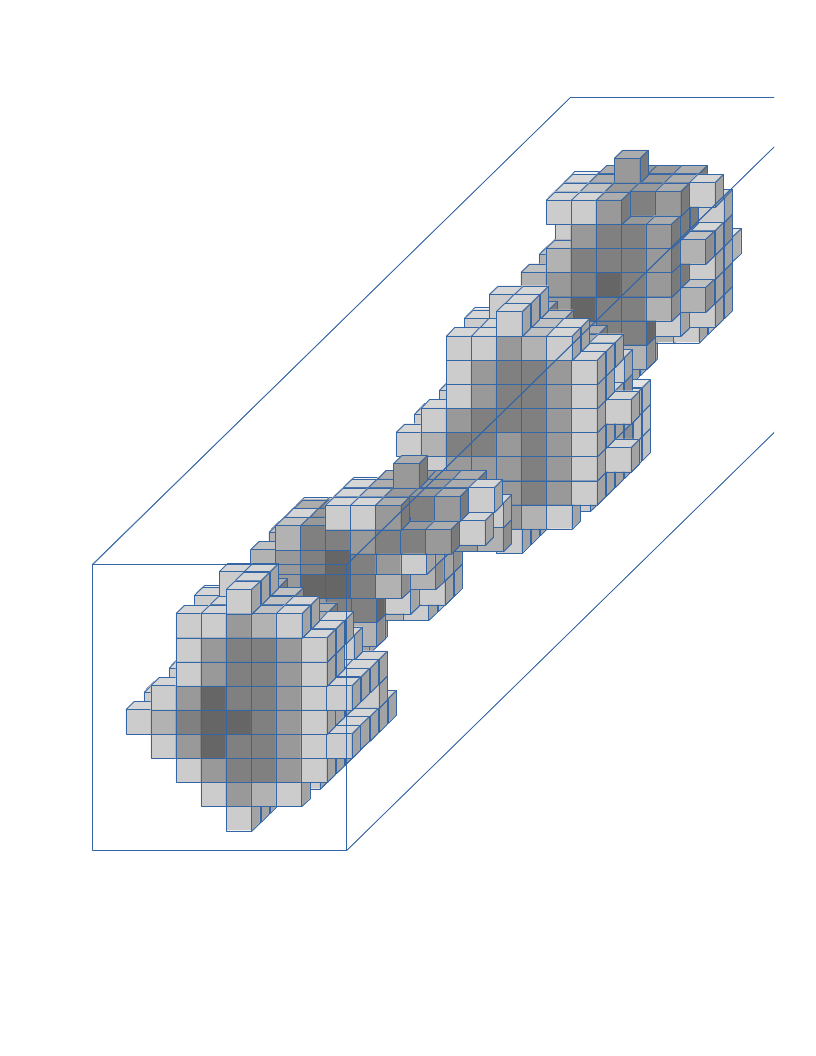
\includegraphics[width=0.7\linewidth]{cube-thresh3.png}}
\end{minipage}
\end{figure}

After defining the sources of the universe, data cubes can be generated by
performing \emph{observations} to the virtual universe, by providing
the following parameters:
\begin{itemize}
     \item Angular central position ($\alpha$,$\delta$), angular resolution $\Delta\theta$ and the Field of View (FOV)
     \item Central frequency $\nu$, spectral resolution ($\Delta \nu$) and spectral bandwidth (BW)
\end{itemize}

The main idea is that each model object knows how to project itself into a
specific data cube depending on its parameters and local definitions. This
allows, for example, generating cubes for the same region but with different
resolutions and/or bands.

\subsection{Functions and Tools for Models}

\begin{itemize}
\item Spatial structures
   \begin{itemize}
      \item Gaussian 2D
      \item Generalized Gaussian 2D (saturated, Lorenzian, etc)
      \item Exponential
      \item Soft-edge rings (TODO)
      \item Random Clouds (TODO)
   \end{itemize}
\item Spectral form
   \begin{itemize}
     \item Skew-Normal Distribution (1D)
   \end{itemize}
\item Local shift functions
   \begin{itemize}
     \item Linear
     \item Exponantial
   \end{itemize}
\end{itemize}

ASYDO implements an example model for generating Interstellar
Molecular Clouds (IMC), 

\subsection{FITS}
\begin{itemize}
\item A 3D image (cube)
\item For each component (and subcomponent) we have
\begin{itemize}
   \item 2D images with the original matrices
   \begin{itemize}
      \item Temperature ($T_m$)
      \item Red-shift ($Z_m$)
      \item Broadening ($\Phi_m$)
   \end{itemize}
   \item A FITS table with each line of the component
   \item This include:
   \begin{itemize}
      \item unique line code
      \item molecule name
      \item chemical name
      \item rest frequency
      \item observed frequency
      \item base red-shift
      \item temperature
   \end{itemize}
 \end{itemize}
 \end{itemize}

\section{Simple Examples}

In this section, we want to highlight two examples of 
how ASYDO can be used.

\subsection{The SVM Hammer}
The Support Vector Machine (SVM) classifier is a popular technique
that allows learning...
\begin{itemize}
\item Pick a 2GHz frequency window ($\sim$ 300 GHz)
\item Select randomly (p=0.3) if a cube have a molecule
\item Force Phosphapropynylidyne existence and abscense (Binary Class)
\item 30000 cubes, 10x10x100 size each ($\sim$ 2 hours)
\item 30000 cubes, 25x25x1000 size each ($\sim$ 4 hours)
\item Naive approach: Use a SVM to train and test (3/4 vs 1/4)
\item Both experiments near 62\%
\item Something is there, but the ML approach is insanely simple
\end{itemize}

\subsection{Line Identification}


\begin{figure}
\centerline{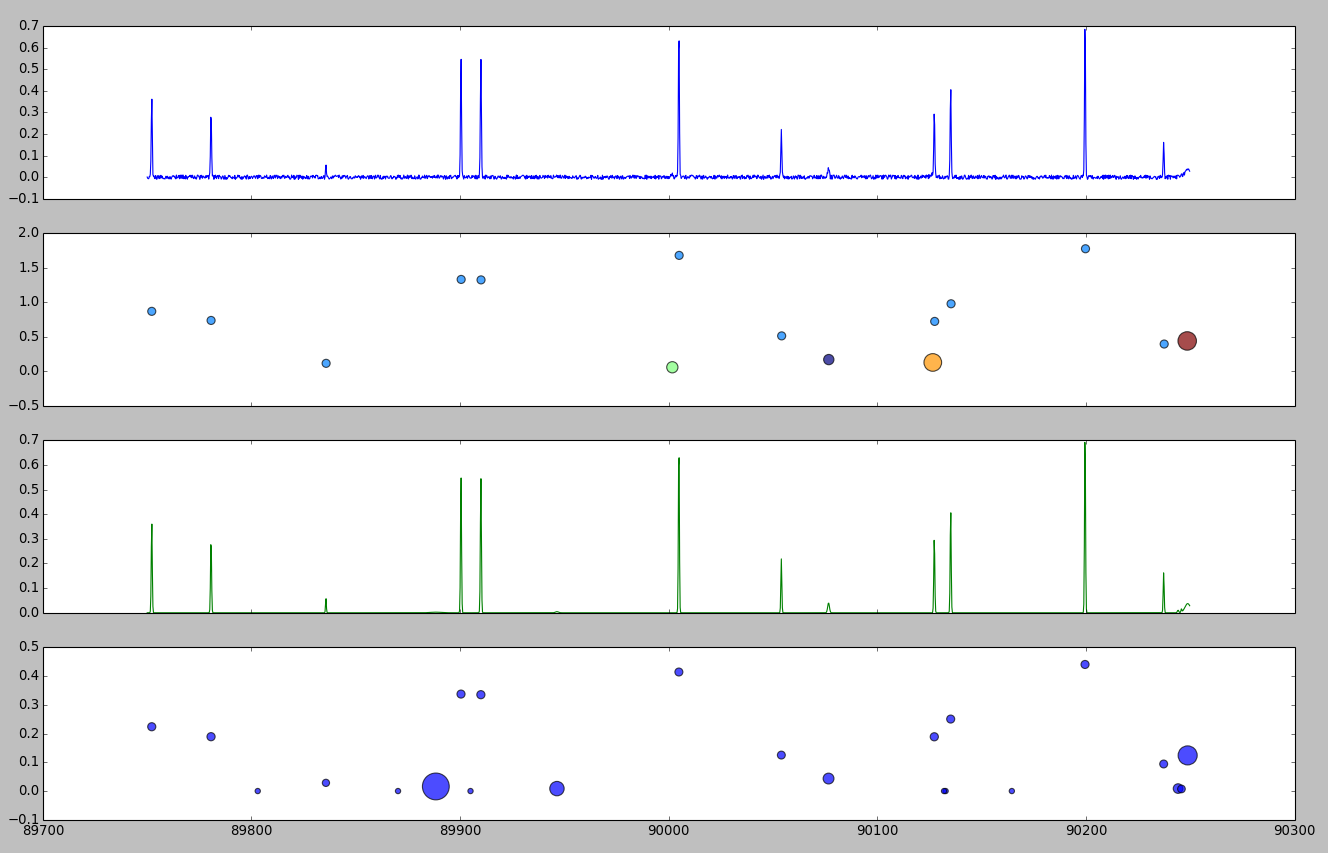
\includegraphics[width=0.95\linewidth]{good_fit.png}}
\centerline{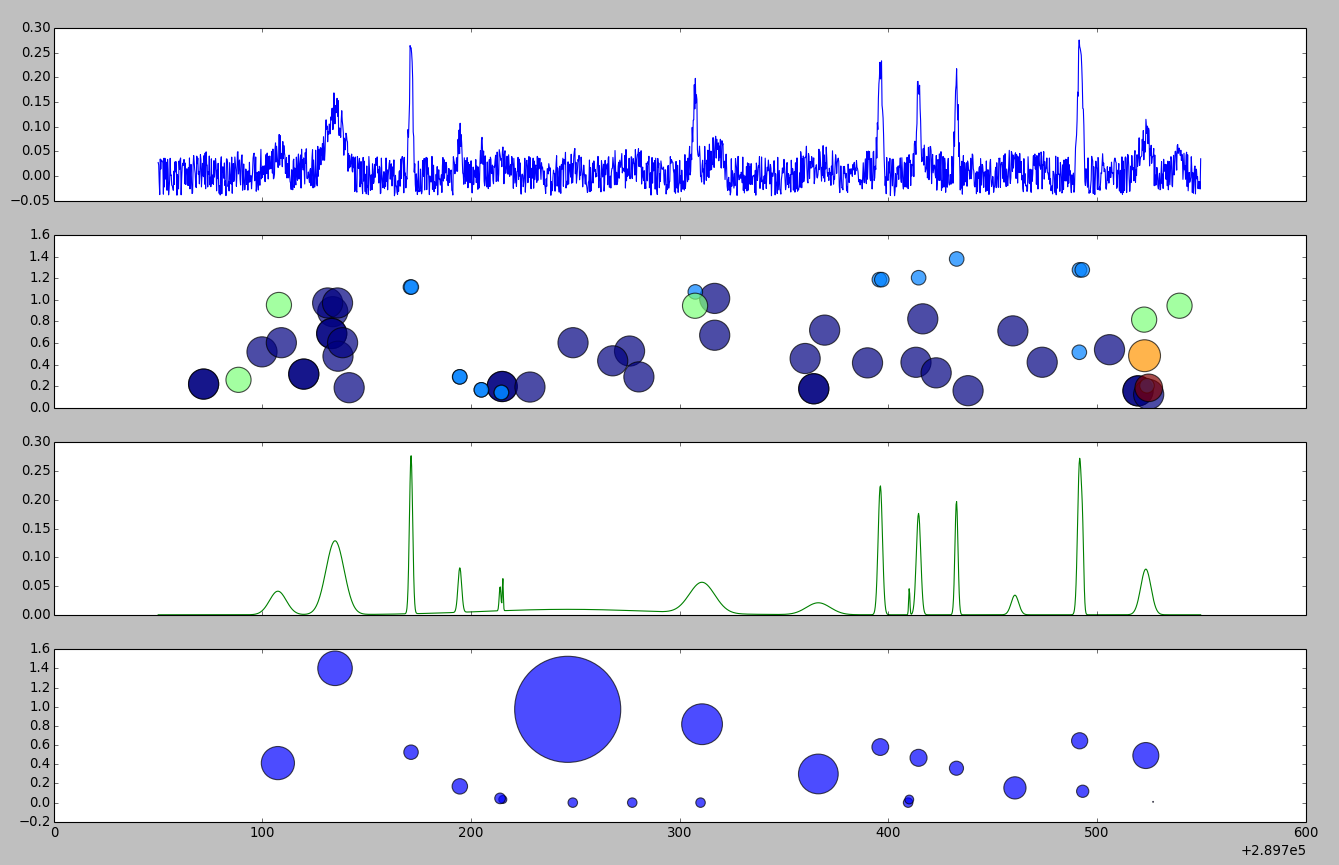
\includegraphics[width=0.95\linewidth]{toomany_fit.png}}
\end{figure}

\section{Conclusions and Future Work}

\begin{itemize}
\item Integration with astropy 
\item IVOA-like synthetic data generation standard (web)
\item Increase the generation speed and improve parallelization
\item Include more models and tools
\item Train using \textbf{synthetic data}, test using \textbf{real data}
\end{itemize}


%\section{The Template}
%To fill in this template, make sure that you read and follow the ASPCS Instructions for Authors and Editors available for download online.  Hints and tips for including graphics, tables, citations, and other formatting helps are available there.
%
%\subsection{The Author Checklist}
%The following checklist should be followed when writing a submission to a conference proceedings to be published by the ASP.
%
%\begin{itemize}
%\checklistitemize
%\item Article is within page limitations set by editor. 
%\item Paper compiles properly without errors or warnings.
%\item No fundamental modifications to the basic template are present, including special definitions, special macros, packages, \verb"\vspace" commands, font adjustments, etc. %(� 3.3, p. 10)
%\item Commented-out text has been removed. %(� 3.3, p. 10,11)
%\item Author and shortened title running heads are proper for the paper and shortened so page number is within the margin. %(� 3.1, p. 4)
%\item Paper checked for general questions of format and style, including, but not limited to, the following:
%\begin{itemize}
%  \item capitalization, layout, and length of running heads, titles  and \\sections/subsections;  % (� 3.1, p. 4) (� 3.2, p. 5) (� 3.3, p. 8)
%  \item page numbers within margin; % (� 3.1, p. 4)
%  \item author names spelled correctly and full postal addresses given; % (� 3.2, p. 5-6)
%  \item abstracts; % (� 3.2, p. 7);
%  \item all margins---left, right, top and bottom; % (�3.1, p. 4; �3.2, p. 5; �3.3, p. 9; �3.6, p. 21);
%  \item standard font size and no Type 3 fonts; %(� 3.3, pp. 10-11; � 3.6, p. 23; � 4.2, p. 25);
%  \item spacing; % (� 3.3, pp. 9-10);
%  \item section headings. % (� 3.3; p. 8).
%\end{itemize}
%\item All tables are correctly positioned within margins, are properly formatted, and are referred to in the text.  %(� 3.5, pp. 16-20)
%\item All figures are correctly positioned within margins, are minimum 300 dpi resolution, not too dark or too light, do not contain embedded fonts, and are referred to in the text.  All labeling or text will be legible with 10\% reduction.  Questionable images printed, checked and replaced if necessary.  Figures do not cover text or running heads, and proper permissions have been granted and acknowledged.  %(� 3.6, pp. 21-24)
%\item All acknowledgments and discussions are in proper format.  % (pp. 11-12, p. 20)
%\item If there are acknowledgments at the end of the article, ensure that the author has used
%the \verb"\acknowledgments" command and not the commands
%\\ \verb"\begin{Acknowledgments}", \verb"\end{Acknowledgments}".
%Acknowledgments should only be used for thanking institutions,
%groups, and individuals who have directly contributed to the work.
%\item All references quoted in the text are listed in the bibliography; all items in the bibliography have been referred to in the text.  % (� 4, pp. 24-28)
%\item All bibliography entries are in the proper format, using one of the referencing styles given. Each of the references is bibliographically complete, including full names of authors, editors, publishers, place of publication, page numbers, years, etc. % (�� 4.2-4.3, pp. 25-28)
%\item A complete Bib\TeX\ file is ready to submit to the editor.
%\item References to preprints replaced with publication information when possible.
%\end{itemize}

\acknowledgements The ASP would like to the thank the dedicated researchers that are publishing with the ASP.

\bibliography{aspauthor}

\end{document}
